\documentclass{article}
\usepackage[utf8]{inputenc}
\usepackage{courier}
\usepackage{graphicx}
\usepackage[numbers]{natbib}
\usepackage{listings}

\lstset
{ %Formatting for code in appendix
    basicstyle=\footnotesize,
    numbers=left,
    stepnumber=1,
    showstringspaces=false,
    tabsize=1,
    breaklines=true,
    breakatwhitespace=false,
    frame=tb
}

\title{Software Evolution: Series 2 Design Document}
\author{Matt Chapman, Dennis van der Werf}

\bibliographystyle{plainnat}
\begin{document}

\maketitle
\section{Introduction}

This document serves as a basic design document accompanying the creation of the \textit{series 2} assignment deliverable: a working clone detection tool with visualisation of clones.

The goal of this document is to explain the basic workings of the tool, along with some rationale for the design decisions that were taken during development.

\section{Using the tool}
To begin using the tool, open the project in Eclipse, and begin a Rascal console session. In this console run the commands \texttt{import CloneVisualisation; runTool();} to start the tool.

In the top right corner of the screen there is a combobox for selecting one of two different projects: \texttt{hsqldb} or \texttt{smallsql}\footnote{In it's default state, the clone highlighting in this project will not work correctly with the tool, due to it using \texttt{CR NL} for new lines. These characters are ignored when files are read by Rascal, but not when creating \texttt{loc} objects. It is necessary to write a script to handle replacing these characters - which will be made available in the project repository.}. Select one of these projects and click \textit{Analyse} to begin the analysis.

Figure \ref{fig:shot1} shows an example of the view presented when a project is analysed. The top bar (green) displays some basic clone metrics for the project in question, along with links that can be clicked to display the biggest clone and clone class.\newpage

\begin{figure}[h]
\centering
\fbox{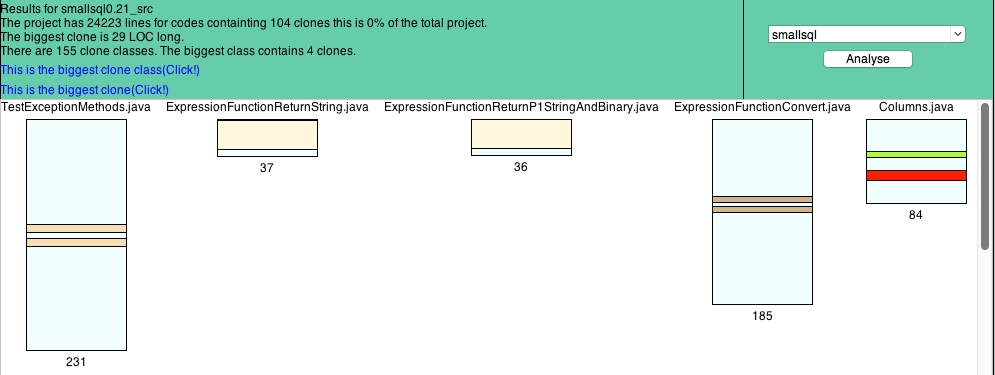
\includegraphics[width=\linewidth]{images/duplicatevis}}
\caption{Duplication Visualisation}
\label{fig:shot1}
\end{figure}

The main view shows each file in the analysed project, with the file name listed above a box that is scaled according to the true size of the file. Under each box is the total file size in LOC (Lines of Code), albeit after the file has been filtered for comments and white space.

Clones are rendered as overlapping, colour coded boxes. Each clone class is rendered in a unique colour, and boxes of the same colour can be assumed to be members of the same clone class. Clicking on a clone class will render only the locations in which the clone class exists. The top bar will display metrics pertaining to the clone class in question.

\begin{figure}[h]
\centering
\fbox{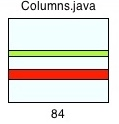
\includegraphics[width=4cm]{images/visexample1}}
\caption{An example file with 2 clone classes}
\label{fig:shot2}
\end{figure}

The files are sorted such that the files containing the largest clones are rendered first on the left. The files containing the smallest detected clones are on the far right of the visualisation.

Clicking on an instance of a clone class within this view will then open the file, with the clone itself highlighted in the editor. Clicking multiple clone instances will open multiple editor instances for easy comparison and verification of detected clones.

Clicking \textit{return to overview} will return you to the start screen, where the entire project is displayed.

\section{Design Rationale}

This section discusses the major design decisions, as well as providing a basic explanation of the algorithm used for clone detection.

\subsection{Satisfied Maintainer Requirements}

As stated in the paper \textit{Cognitive design elements to support the construction of a mental model during software exploration} by \citeauthor{Storey1999171}, there are a number of possible requirements that a maintainer may have of a software tool. We believe that the tool we have created satisfies the following requirements\cite{Storey1999171} from this paper, in the following ways:

\begin{itemize}
\item \textbf{Improve Program Comprehension}: We fulfil this requirement by providing top-down comprehension facilities through the use of generalised statistics and metrics, and also through the visualisation itself. As the visualisation is very much a ``top down'' view of the analysed project, and shows an easy to read summary of detected clones through colour coded notation, we believe that this requirement is fulfilled.
\item \textbf{Facilitate Navigation}: We have made the visualisation (and indeed some of the basic metrics) interactive. By clicking the rendered clones, the user can navigate backwards and forwards through varying \textit{depths} of views, from an overall project view, to clone classes, to the clones themselves.
\item \textbf{Reduce Disorientation}: By implementing our visualisation natively in Rascal using the \texttt{Vis} library, we have successfully minimised maintainer disorientation. The visualisation is rendered directly in a tab contained within Eclipse, and also opens all files (when the user instructs it to do so) in the Eclipse native editing environment - with the clone conveniently highlighted. We also ensure that views are re-used where possible, to prevent an overload of tabs and other windows building up.
\end{itemize}

\subsection{Clone Detection Algorithm}

\begin{lstlisting}[caption=Clone Detection Algorithm,label=lst:algorithm]
Function detectClones(project)
{
    for(every file in project)
    {
        filter comments & white space;
        get first 6 lines of filtered file;
        hash first 6 lines;
        
        if(first 6 lines already in clone set)
            mark as duplicate;
        else
            add to clone set;
    }
    
    for(every file in project)
    }
        while(first duplicate is still a duplicate)
        {
            grow duplicate bounds by 1 line;
        }
        
        flag subsumed clones;
        
        remove subsumed clone classes;
        
        for(every other duplicate in file)
        {
            while(duplicate is still a duplicate)
            {
                grow duplicate bounds by 1 line;
            }
        }
        
        re-filter for subsumed clones;
        write results to file;
        render the results;
    }
}
\end{lstlisting}

The listing above (Listing \ref{lst:algorithm}) shows the basic pseudo-code behind the clone detection algorithm that we are using.

This algorithm works by detecting \textit{Type 1} clones, that is ``Identical code fragments except for variations in white space (may be also
variations in layout) and comments''\cite{cloningsurvey}. While it would be possible to write an implementation for \textit{Type 2} clones (via the use of Abstract Syntax Trees and sub-tree comparison therein) we opted instead to extend, optimise and improve the clone detection algorithm we had in place from our \textit{Series 1} deliverable.

While the pseudo-code in Listing \ref{lst:algorithm} gives a succinct explanation of it's workings, some further explanation follows. The algorithm begins by obtaining all of the source files contained within a given project, and then filtering them to remove white space and comments. These elements are surplus to requirements and should not be considered in any clone detection algorithm. For each obtained and filtered file, we take the first 6 lines of that file and insert it into a map as the key - which makes use of hashing for the key, is much faster than direct string comparison.

If the key (the hashed 6 lines) already exists in the map then we flag it as a clone. Otherwise, it is added to the map structure. Once all files have been examined, the algorithm starts \textit{growing} the first clone in each file, incrementally extending the clone `window' by one line, and checking if this clone now subsumes any others. If it does, then the clone is flagged as a subsumed clone. If all clones in a class are flagged as subsumed then the clone class is removed from the data structure.

This `grow' operation is then carried out on all of the clones to ensure that the clones are as big as possible. The clones are extended by one line at a time, and checked to see if they are still equal. Once one clone or the other in a given clone class is no longer equal, we store the upper bound of the windows size wherein the clones are still equal and move on to the next one.

Once all of the clones have been grown as far as possible, we re-filter for any further subsumed clones (to avoid duplicates). Once this final filtering step is completed, the clones and clone classes are then passed to the reporting and rendering libraries to create the final output of the algorithm.

\subsection{Visualisation}

The text \textit{Identifying and Removing Software Clones} by \citeauthor{Koschke2008} provides several examples of possible clone visualisations.

One visualisation in particular was created by \citeauthor{Tairas:2006:VCD:1188835.1188846} in their tool for \textit{Visualization of Clone Detection Results}\cite{Tairas:2006:VCD:1188835.1188846}.

This visualisation makes use of three component parts, namely \textit{boxes, lines and kinds}. Boxes are the containers representing the files, the lines represent the bounds of the various detected clones, and the kinds are represented by varying colours of the lines.

This type of visualisation (boxes representing files, arranged vertically and overlaid with coloured bars to represent areas of the file) also appears several times in the lecture slides \textit{Towards Visual Software Analytics} by Paul Klint\cite{klintslides}.

Being that our aim was to create a tool for a maintainer, as opposed to just blindly print out metrics, we opted to reproduce this visualisation using the Rascal \texttt{Vis} library. There were certainly other options available to us (namely various JavaScript libraries with ``pre-baked'' visualisation options that only require the ``plugging in'' of existing data, though there were two main reasons that we did not take this avenue:

\begin{itemize}
\item \textbf{Maintainer requirements:} As stated in a previous section, our intention was to meet the requirement of reducing maintainer disorientation. If we utilised an external library (as opposed to the Rascal library - which renders its results directly in Eclipse) then it was likely that the maintainer would have to leave their IDE in order to view results, thus rendering our attempt to minimise maintainer disorientation somewhat pointless.
\item \textbf{Platform Familiarity:} While using an established Javascript library could be viewed by some as the ``easy option'', the fact that we were already familiar with Rascal as a platform meant that the ``educational overhead'' of learning to use the Rascal \texttt{Vis} library was far lower than attempting to implement visualisation in Javascript.
\end{itemize}

The built-in Rascal libraries do offer the possibility of using the \texttt{Outline} object to create visualisations such as this. Unfortunately the existence of this object came far too late in the development process to be of any use, and as such the process below become a valuable \textit{learning experience} regarding reading documentation and planning before beginning an implementation.

Our visualisation starts by generating a box for a given file. This box is of fixed width and it's length is bounded by the length of the file itself. Once this container is created, we create a list of boxes, one for each clone contained within the file. These boxes are again of fixed width, and bounded by the length of the clone they are going to represent. As we know the start line of any given clone, they are aligned vertically using \texttt{FProperty valign(n)} where \texttt{n} is set according to how far through the container file the start line of the clone is situated. These boxes are then added to a list and overlaid on the container box, which is in turn added to a \texttt{vcat} object along with the file name and file length. These figures are then added to a \texttt{hcat} object which contains all of the completed figures.

\section{Caveats}
\subsection{Known Issues}

\begin{enumerate}
\item There is some evidence to suggest that the \textit{filtering} algorithm used to strip comments and whitespace before running the clone detection algorithm, does not produce perfect results. Indeed we have noticed that there are some styles of multi-line comment that the regular expression we are using may not catch in certain situations.
\item The clone detection algorithm only detects \textit{Type 1} clones at this time. Future iterations would make use of Abstract Syntax Trees and subtree comparison to detect \textit{Type 2} clones, but time constraints lead us to extend our existing \textit{Type 1} detection algorithm rather than beginning a new implementation.
\end{enumerate}

\newpage
\bibliography{evo.bib}

\end{document}
